%!TEX root = ../dissertation.tex

\begin{savequote}[0.6\textwidth]
	\itshape I suppose it is tempting, \\
	\itshape if the only tool you have is a hammer, \\
	\itshape to treat everything as if it were a nail.
	\qauthor{---Peter H. Salus}
\end{savequote}

\chapter{Introduction}
\label{chap:01}

\Lettrine{Molecular} modeling and simulation, defined as the use of \textbf{computational methods to describe the behavior of matter at the atomistic or molecular level},\cite{maginn2009} comprises a large array of software designed to solve very different problems in wide areas of molecular biology and theoretical chemistry: characterization of reaction profiles, drug discovery, optimization of catalytical processes$ \ldots $  A good modeler knows which techniques and theories must be applied depending on the task at hand, which is even more difficult if one has to take into account the software diversity. Just choosing where to begin can be a daunting task.

This introductory chapter will provide a brief overview on: (1) the major software categories in molecular modeling, which will be further detailed in \autoref{chap:02}; (2) how they can be used together in integrative approaches; and (3) the difficulties, caveats and pending challenges present in these approaches.

\section{In silico molecular modeling}
% \addcontentsline{toc}{section}{In silico molecular modeling}
\subsection{Overview of molecular modeling tools}
% \addcontentsline{toc}{subsection}{Overview of molecular modeling tools}

After decades of development, the number of readily available computational tools can be overwhelming. Depending on the phenomena studied, different techniques are more appropriate than others. This section only provides an overview on the fields and hills that populate the current landscape. A more detailed description on the available techniques can be found in \autoref{chap:02}.

The most popular task performed in molecular modeling consists of describing the energetics of a system, which can then be used as a proxy for structure optimization, reaction path guessing or studies on dynamic behavior, among others. Depending on the method employed to obtain those energies, the results will resemble the experimental observations with higher or lower accuracy.

Atop the accuracy curve we can find Quantum Mechanics (QM) methods, which are based on quantum chemistry and the equations proposed by Schrödinger in 1925. This family of methods consider electrons explicitly, which allows them to study chemical reactivity with highest precision. However, given the complexity of the calculations involved, even modern hardware cannot deal with more than a few hundred atoms.

The next major family, Molecular Mechanics (MM), discards electronics for the sake of speed and scale. Instead of applying Schrödinger’s theory, it considers molecules as a set of spheres connected by carefully calibrated springs, whose energy is given by Newton’s laws of motion. This results in much simpler calculations which can deal with thousands of atoms almost instantaneously. In fact, their most popular usage is its time-dependent implementation, Molecular Dynamics (MD), which analyzes the evolution of a system over millions of timesteps to obtain an accurate representation on the molecular behavior along a few nanoseconds.

QM and MM can be used simultaneously in the same system using an approach called QM/MM. This hybrid method allows to consider larger structures by splitting the calculations in two regions modeled differently. QM is applied to a reduced part of the system that requires an accurate electronic representation, while the rest of the structure is processed with the simpler MM techniques. Both calculations are then integrated by using hybrid schemes such as IMOMM $ \{ $ $ \} $ , IMOMO $ \{ $ $ \} $  or, most popularly, ONIOM $ \{ $ $ \} $ .

Even though it can be argued that energy calculations are behind every molecular modeling study, not all methods focus on obtaining an accurate value. Sometimes, a distantly close one is enough. For example, protein-ligand docking studies are designed to obtain probable orientations in which a small molecule (ligand) can bind to a bigger one (protein). For this assessment, obtaining an accurate binding energy is not as important as navigating the search space reliably: it is preferred to focus on the fast generation of reasonable candidate poses instead of a locating a true global minimum. To\ do that in an affordable time, accurate energies are normally replaced by scoring functions that return pseudo-energies or even unitless scalars. These functions can be based on simplified molecular mechanics, knowledge-based potentials, shape complementarity or even simple geometric measurements.

Drastic simplifications of energy are not uncommon in molecular modeling, especially if large search spaces must be analyzed efficiently. Normal Mode Analysis (NMA) apply an even simpler ball-and-springs model to obtain the principal vibration frequencies of a molecular structure. Under this approach, collective motions can be assessed in minutes without resorting to long molecular dynamics, which can take days or weeks to finish.

Vast search spaces are not limited to macromolecules with large number of atoms. Every variable considered during an analysis generates an additional dimension in the search space. Any slight change in the topology of the molecule can incur in more complexity, such as exploring point mutations in the protein sequence (biological space) or testing different functional groups in one part of the ligand (chemical space). Exploring (bio)chemical spaces require very specific tools and there is no general-purpose utility in that regard. For chemical spaces, QSAR (for Quantitative Structure-Activity Relationship) can be applied: these are classification or regression methods that can predict chemical properties of a compound (like biological activity of a drug) by relating key properties in big datasets (presence of certain functional groups, for example).

Regardless what method is finally applied, any software will always need input information to work with. Depending on the tasks to perform, the required data can range from simple geometry specifications, to connectivity, atom types, charges, spin state, temperature, optimization steps or algorithmic treatment. While helper software exists, it is the user’s responsibility. In some cases, it will be as trivial as downloading a file from a database, but in others it can be more difficult. Carrying out these tasks efficiently is also part of the skillset expected of a molecular modeler and will be further discussed in \autoref{chap:02} and \autoref{chap:03}.

\subsection{Multiscale and integrative modeling}
% \addcontentsline{toc}{subsection}{Multiscale and integrative modeling}
Multidimensional search spaces are hard to navigate with a single method, so most popular approaches resort to multistep protocols that recruit different techniques along the process. This adds one more challenge to the scientific work: putting all the software to work together.

Multiscale modeling is often necessary because many molecular phenomena comprise a wide range of magnitudes at different scales. The covalent bond of a hydrogen atom stretches at a frequency of 1ps, but other harmonic vibrations can take up to nanoseconds in macromolecules where collective motions are present. A key cofactor in a new catalysis method can be comprised of less than 10 atoms, while proteins and nucleic acids that develop critical functions in our cells can be made of tens of thousands. Some studies like enzyme inhibition, biocatalysis or artificial metalloenzymes often require looking at both sides of the scale to obtain valuable information.

This is hard because the bigger a system is and slower the phenomena, less accuracy can be afforded in reasonable time periods. Highly accurate methods like quantum mechanics are usually disregarded when more than 500 atoms are considered. Faster methods like semi-empirical approaches to QM or polarizable molecular mechanics can help in bigger systems, but at the cost of less accuracy. Following that trend, mesoscale methods stop considering atoms individually altogether and group them in coarse-grained entities. If possible, they can also take great advantage of the existing symmetry in the structures under study.

The consequences of having different methods for different size and timescales is that those methods must be combined in well-designed hybrid protocols. There is no clear strategy that dictates the proper sequence of methods and levels of theory. Most common protocols start with less accurate methods like docking, select some poses for further assessment using MD simulations, and pick some representative states frames to be optimized in QM or QM/MM schemes $ \{ $ $ \} $  (see fig. \ref{fig:multiscale}). However, depending on the information available, a study can begin with a DFT optimization of a reduced model and then progressively consider more atoms by decreasing the method accuracy: freezing some atoms in a cluster model, using semi-empirical approaches or hybrid methods and finally checking stability with a MD simulation $ \{ $ $ \} $ .

Every study is different and presents unique scientific and technical challenges, which are almost always overcome on an individual basis. Workarounds, patches and scripts are so commonly needed that it becomes an art on its own. In the future, this will be less of an issue as hardware gets faster and software smarter, but in the meantime standardizing some common workarounds can produce successful results.



\begin{figure}[H]
		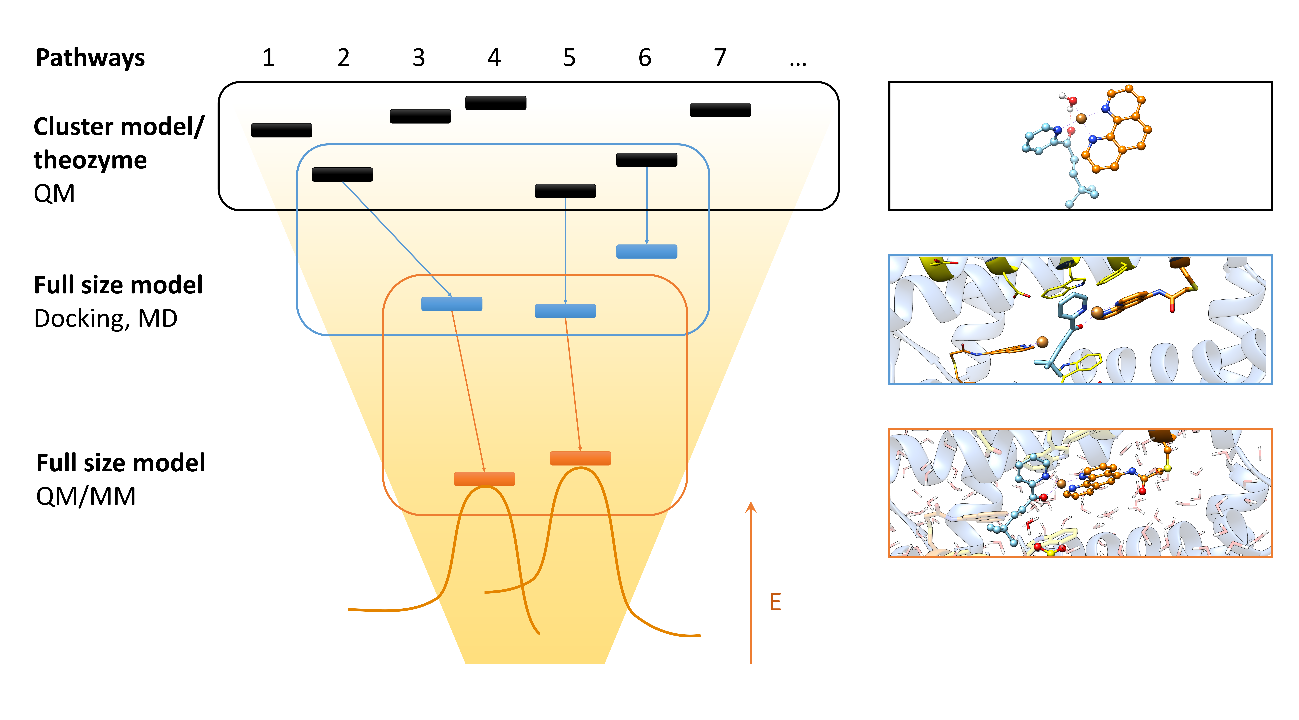
\includegraphics[width=\textwidth]{./figures/01/multiscaleprotocol.png}
		\caption[Example of a multiscale protocol]{Example of a multiscale protocol applied for the identification of the catalytic mechanism of a metallic cofactor inside a metalloenzyme.\cite{victor2014} (Reproduced from Simulating Enzyme Reactivity : Computational Methods in Enzyme Catalysis., Chapter: 15, Publisher: The Royal Society of Chemistry, Editors: Iñaki Tunon, Vicent Moliner, p. 514).}
		\label{fig:multiscale}
\end{figure}


\section{Unresolved and challenging issues and how to deal with them today}
% \addcontentsline{toc}{section}{Unresolved and challenging issues and how to deal with them today}
Even though the horizon might look like exciting, we still must solve some issues in the current state of the art. Only by providing solid foundations we will be able to build a strong future. In molecular modeling, problems may arise anytime during the full process. Missing structural data, lack of parameters or software incompatibilities are the most common issues and will be detailed in the following points.

\subsection{Dealing with software fragmentation}
% \addcontentsline{toc}{subsection}{Dealing with the software fragmentation in molecular modeling}
The vast landscape of molecular modeling is comprised of hundreds of programs that have been developed to address different problems and, most of the time, with only that problem in mind. They were not designed to be part of a bigger, integrated workflow. This is important because few computational studies are composed of only one step that relies on a single program to obtain a one-shot result after the first calculation. They usually comprise multiple stages that combine several theory levels and software packages to achieve the intended results. This is especially true in multiscale approaches, as pointed out by Grimme and Warshel (see \autoref[Appendix]{chap:appendix-a}). Subsequently, good integration is needed between the involved software, which unfortunately, it is not always the case.

Each of the steps will require different information depending on the supporting theory (in addition to atoms and coordinates, some will need connectivity, residue grouping, charges, parameters) and each of the involved programs might exhibit slight differences in how the exchanged files are parsed or exported. For example, one particular tool handles element names as case-independent, while the next one would only accept uppercased names, or use different unit systems and a conversion is required (nanometers and angstroms is a common one). As a result, even after managing to correctly thread the needed file formats as required, a robust behavior of the workflow is not guaranteed and ends up in fragile, unexpected performance.

This is both cause and consequence to the absence of a standard file format to deal with biomolecules and chemical compounds. On the contrary, the first programs created custom file formats to deal with their own necessities, which has led to several file formats coexisting with an overlapping set features. XYZ is the simplest, with only providing a list of elements and their coordinates, line by line; crystallographers use PDB files to handle big macromolecular structures such as proteins; MDL (now part of Dassault Systems) created MOL and SDF files to deal with small compounds; Tripos’ Sybyl (now part of Certara) introduced MOL2 for their docking studies$ \ldots $  only to name a few.




After so many years of battling the file format war, a true standard is yet to be defined. While there are ongoing efforts trying to solve part of the issue --the crystallographic community is slowly replacing the troublesome PDB file format with mmCIF--,\cite{bourne1997,berman2007}) new developments still have to deal with multiple input and output files to be competitive (see fig. \ref{fig:xkcd}). Some projects exist to cover the compatibility issues, such as the popular OpenBabel suite, \cite{oboyle2011} but that constitutes only a band-aid and not a true solution.

\begin{figure}[H]
	
\includegraphics[width=\textwidth]{./figures/01/xkcd927.png}
	\caption[Proliferation of standards]{How standards proliferate. Reproduced from XKCD 927 (www.xkcd.com).}
	\label{fig:xkcd}
\end{figure}


\colorbox{yellow}{ [Other problems to mention?]}

The solution to this fragmentation is not an easy feat, and several strategies could be implemented to alleviate the issue. The first milestone is, simply put, write good documentation: time-tested protocols, which detail the software and versions used in each step are of utmost importance. If files need to be exchanged and/or edited along the process, these editions must be noted too. Of course, multiscale protocols are only a patch and do not solve the background problem: fragmentation. In this matter, several software-only attempts have been made throughout last decades and will be further detailed in \autoref{chap:05}.

\subsection{Missing or partial structural data}
% \addcontentsline{toc}{subsection}{Missing or partial structural data}
modeling a compound or structure usually requires a good enough starting point, which depends on the type of structure. For example, building a small molecule like a drug or a catalyst has nothing to do with obtaining a macromolecular structure.

To work with small compounds, researchers usually draw a 2D depiction in software like ChemDraw $ \{ $ $ \} $  and then obtain a 3D structure out of it. Sometimes, the 2D->3D conversion is not trivial and a 3D model is sketched by hand in GaussView $ \{ $ $ \} $ , Avogadro $ \{ $ $ \} $  or similar software. $ \{ $ $ \} $  The automatic procedures are good enough to provide a reasonable structure, but more often than not the final structure has been manually adjusted. If the system features many degrees of freedom, this can be tedious. A common alternative consists of performing high-temperature molecular dynamics simulations to navigate the conformational landscape. Once the researcher is satisfied, the small compound can be directly minimized with quantum mechanics algorithms, but if the size is too large a short MD run might be required instead, in this case to ‘relax’ the structure.

Manually building molecules is feasible when the number of atoms is reasonable, but with macromolecular structures such as proteins or DNA this does not hold true. For this type of systems, the initial model will ideally come from experimental data such as atomic-resolution 3D coordinates obtained with X-Ray crystallography (XRC) or Nucleic Magnetic Resonance (NMR). However, even if a 3D model is available, a part of the structure can be missing, which is very common with flexible loops. If that is the case, the researcher must model the missing parts by rebuilding the known sequence with sensible spatial restraints. In other cases, the full 3D structure might be missing, but similar structures (homologs) are available and can be used as a template -the perfect application for homology modeling (see \autoref{chap:02}). In both cases, the resulting structures should be quality-assessed with utilities like ERRAT $ \{ $ $ \} $  or PROSESS $ \{ $ $ \} $ . Sometimes, MD simulations are needed to check if the structure is stable along time, which can be also recommended in some other cases like XRC models with high B-Factors or deviant multi-model NMR structures.

Even with a proper protein structure, if the study features custom ligands, obtaining a good candidate for further steps in the protocol is not as simple as one might think. Assuming the required ligand structure is available, a regular protein-ligand docking simulation can provide an initial guess of the complex, but this is usually processed with long MD runs to assess the stability of the interactions. However, if the ligand is not known and must be designed from scratch, there is no consensus strategy. Two common approaches involve: (1) creating a library out of ligands that exhibit the needed chemical features using a reverse pharmacophoric approach, which then would be screened to assess their stability within the protein; (2) applying topology operators during the docking simulation itself using topology operators to dynamically build the ligand out of smaller fragments. The latter has been applied successfully in one the programs presented in this thesis, and will be discussed in \autoref{chap:06}.

For larger scale systems like viral capsids or lipid bilayers, which can feature millions of atoms, building a starting structure can be daunting at first, but fortunately they all exhibit some kind of symmetry that can be used to assemble the full structure out of the involved subunits with specialized software. $ \{ $ $ \} $

\subsection{Living with metal ions in macromolecules}
% \addcontentsline{toc}{subsection}{Living with metal ions in macromolecules}
One of the most exciting areas of molecular modeling sits at the frontier between organometallics and biochemistry, two fields that have been studied separately in computational chemistry for decades now. Globally, chemists exploit their features differently and, as such, present different computational challenges. Traditionally, organometallic systems feature a reduced number of atoms and accommodate transition metal centers within their structure, whose exotic electronic behavior can only be accurately computed with quantum chemistry approaches. Studies on biological problems such as the early work on folding of peptides and proteins had to face a larger number of atoms (hundreds or thousands) from the beginning, forcing the authors to use classical mechanics approaches to deal with the added dimensionality after realizing that the electronics of the system were not very important in that process.

However, metals do take part in biological processes as mainstream as oxygen transportation and muscle contraction. As such, the existence of metalloproteins cannot be neglected by the modeling community, who should bring these two areas together in a more seamless experience. Given the diverging efforts accumulated for decades, the gap is not easily overcome, but some solutions exist. Depending on the properties to study, one can resort to different approaches, as detailed below.

\subsubsection{Quantum Mechanics}
% \addcontentsline{toc}{subsubsection}{Quantum Mechanics}
Since quantum mechanics deal explicitly with the electronic shells of atoms, the immense diversity of electronic configurations of metal ions does not represent a problem. If such, the only challenge this might present is choosing the adequate functionals, basis sets or starting-point structures.

The challenge is more technical than scientific. While advances in DFT theories and hardware architectures allow us to deal with up to 500-atom systems in feasible timescales, this is still far from the number of atoms usually present in protein structures. For this, hybrid QM/MM studies are more adequate: the QM layer is responsible for dealing with the metal and its surroundings (at least, the first coordination sphere), while the, comparatively cheap, MM layer governs the rest of the structure. Even with this approach, time-dependent schemes still represent a huge computational effort, not to mention the difficulties in setting up the system adequately. One must still deal with layer boundaries effects or the parameterization needed for the MM calculations.

\subsubsection{Molecular Mechanics}
% \addcontentsline{toc}{subsubsection}{Molecular Mechanics}
Sometimes, QM is not necessary for a modeling study, since the metal might only play a structural role without exhibiting reactivity. In these cases, it is more interesting to gather an insight into the structural behavior of the system along time. Nowadays, for macromolecular systems, this is only feasible with molecular dynamics approaches, which require accurately parameterized force fields. Traditionally, force fields were developed to solve problems existing with proteins, nucleic acids and organic compounds $ \{ $ Lifson, Allinger, and so on; lots of references in the UFF paper$ \} $ , so historically transition metals have not been considered in force field development. Additionally, they present complexities not present in the reduced set of organic elements: several coordination geometries, different charge states, exotic polarizable behavior... As a result, dealing with metals in molecular mechanics is usually challenging. One must choose between (1) not considering them at all, (2) using a low-accuracy general-purpose force field, or (3) facing the tedious process of parameterization.

Ignoring or removing the metal ions can be acceptable in certain cases where they do not play a crucial role in the structure or dynamics of the system, but that is rarely the case. While general purpose force fields are numerous and heavily used, they mostly target organic compounds (such as CGenFF,\cite{Vanommeslaeghe2009} GAFF,\cite{Wang2004} Tripos 5.2 force field\cite{clark1989}). Only some include parameters for metal ions: UFF (for Universal Force Field,\cite{rappe1992} MMFF\cite{halgren1996}) covers the full periodic table, but Dreiding\cite{Mayo1990} only contains parameters for Na, Ca, Zn and Fe. While useful for organic chemistry, they are not as used in simulations including biological systems $ \{ $ $ \} $ , since they tend to rely on the Lennard-Jones based ‘nonbonded model’ $ \{ $ $ \} $ .

A feasible alternative for bio-containing systems is the so-called ‘bonded model’, which treats metal ion interactions with both bonded and non-bonded parameters; i. e., the metal is assumed to bond to some residues. Some of the protein-oriented force fields like AMBER $ \{ $ $ \} $  or CHARMM $ \{ $ $ \} $  distribute force field extensions for some of the most common metal ions in proteins, such as hemo-coordinated iron, but mainly as examples on how custom parameters can be added in the software. These types of force field extensions are only valid for the context where the parameters were obtained; i. e., the iron parameters for the heme groups will not reproduce the behavior of iron in other organic contexts such as ferrocenes. While the file format is easily understood, the values of the parameters are not easy to obtain: one has to resort to experimental data or \textit{ab initio} calculations to get adequate constants for bonded (distances, angles, dihedrals) and nonbonded (electrostatic, Van der Waals) interactions. While an expert user can decide to obtain those values manually, the process is not trivial and some protocols and tools have appeared to assis. They are mostly based on the Seminario’s method and his FUERZA software, \cite{Seminario1996} such as MCPB, MCPB.py,\cite{li2016} VFDFT.\cite{zheng2016} Recently, alternative approaches based on machine and statistical learning, \cite{fracchia2017,li2017b} and non-Seminario strategies\cite{Burger2012, allen2017} have also appeared, but the principle remains the same: extract the information from \textit{ab initio} calculations. Given the complexity of the task, some specific force fields have arisen lately to provide parameters for certain metals:

\begin{itemize}
	\item \href{http://onlinelibrary.wiley.com/doi/10.1002/9780470125830.ch2/summary}{http://onlinelibrary.wiley.com/doi/10.1002/9780470125830.ch2/summary}

	\item \href{http://onlinelibrary.wiley.com/doi/10.1002/jcc.10171/full}{http://onlinelibrary.wiley.com/doi/10.1002/jcc.10171/full}

	\item \href{http://pubs.acs.org/doi/abs/10.1021/ic00068a012?journalCode=inocaj}{http://pubs.acs.org/doi/abs/10.1021/ic00068a012?journalCode=inocaj}

	\item \href{http://pubs.acs.org/doi/abs/10.1021/jp046244d}{http://pubs.acs.org/doi/abs/10.1021/jp046244d}

	\item \href{http://pubs.acs.org/doi/abs/10.1021/ja00001a001?journalCode=jacsat}{http://pubs.acs.org/doi/abs/10.1021/ja00001a001?journalCode=jacsat}

	\item \href{http://onlinelibrary.wiley.com/doi/10.1002/jcc.20634/full}{http://onlinelibrary.wiley.com/doi/10.1002/jcc.20634/full}

	\item \href{http://onlinelibrary.wiley.com/doi/10.1002/pssb.201248460/full}{http://onlinelibrary.wiley.com/doi/10.1002/pssb.201248460/full}

	\item \href{http://pubs.acs.org/doi/abs/10.1021/ct400952t}{http://pubs.acs.org/doi/abs/10.1021/ct400952t}
\end{itemize}

A radically different strategy consists of mimicking the interactions of the metal site with positively-charged pseudoatoms strategically placed at around 0.9A from the metal nucleus following the vertices of the adequate coordination geometry. The Cationic Dummy Atom Model (CDAM) was introduced for Mn2+ ions by Aaqvist $\&$  Warshel in 1990\cite{aaqvist1990} and has been successfully implemented in further studies fore Zn, Mg, Ca, Fe, Co, Ni, Cu and more $ \{ $ duarte2014, 788, 790-795 in li2017$ \} $ . Among its advantages, once parameterized the CDAM approach is context-independent, but it forces a fixed coordination number and geometry on the modeled metal site.

The application of polarizable force fields (Fluctuating Charge methods, ABEEM, Drude oscillators and rods, induced dipoles, AMOEBA, PFF) or more exotic models based on Angular Overlap and Valence Bond Theory are also promising approaches, but the additional calculations incur in a big performance penalty when compared to other strategies and still require additional parameterization. Further details on the topic can be found in the extensive review published by Li and Merz Jr. in 2017.\cite{li2017}

\subsubsection{Lower levels of theory}
% \addcontentsline{toc}{subsubsection}{Lower levels of theory}
If the study at hand does not require a molecular mechanics treatment, such as docking studies of virtual screening approaches, the parameterization problem is usually not present or, at least, not that complicated. Docking studies, which try to accommodate small compounds within macromolecules, have not considered metals for years, since they were originally designed to find drug-like, organic compounds suitable for the pharmaceutical industry. Fortunately, over time some of the most popular docking packages have included strategies to deal with metals $ \{ $ FlexX$ \} $ , albeit sometimes they could only be part of the host (usually a protein), and not part of the probe (the ligand) $ \{ $ GOLD$ \} $ . To overcome the problem, approaches inspired in the Cationic Dummy Atom Model implemented in MM studies have been designed (‘H-bond trick’): in this case, the dummy atoms are hydrogen atoms that behave as a hydrogen bond donor, a chemical feature commonly implemented in docking software.

Other approaches involve considering the metal problem as a geometric optimization problem, restraining their position with distances, angles and dihedrals measurements. This strategy is partially implemented in homology modeling software like MODELLER, \cite{Sali1993} and is one of the main features of the developments presented in this thesis (detailed in \autoref{chap:03}).

In cheminformatics, explicit consideration of atoms is not as important and strategies like the pharmacophoric studies only have to consider metals as a custom type of interaction hotspot $ \{ $ johns2009,kawasuji2012,carcelli2014.pdf,yang2016$ \} $ . In QSAR, a catalogue of metal empirical properties is enough to build the dataset (QSAR $ \{ $ Fundamental QSARs for Metal Ions, John D. Walker, Michael C. Newman, Monica Enache, CRC Press; December 2012$ \} $ , especially in toxicity studies. \cite{enache2003,can2007,puzyn2011,gajewicz2014,pan2016}.

